\documentclass[11pt]{article}

\usepackage{amsmath}
\usepackage{amsfonts}
\usepackage[margin=1in]{geometry}
\usepackage{enumitem}
\usepackage{graphicx}
\usepackage[colorlinks]{hyperref}
\usepackage{longtable}

\usepackage{helvet}
\renewcommand{\familydefault}{\sfdefault}

\setlength{\parindent}{0in}

\def\tightlist{}
\def\toprule{}
\def\bottomrule{}

\begin{document}
This homework is not ready until this message has been removed.

\section{Homework 2 (Due September
16th)}\label{homework-2-due-september-16th}

Homework 2 emphasizes the electric field and the principle of
superposition that will form the basis of much of your understanding of
electrostatics. This homework makes use of what you learned from Secs.
1.1-1.4 in Griffiths and adds to it the concepts from Sec. 2.1, which
make up the bulk of the assignment. In addition, we have begun to
introduce the idea of finding approximate formulae using Taylor
expansions, which is one of the most common practices of theoretical
physics. In this assignment, you will use a Jupyter notebook to explore
the concept of superposition and visualize the field of a charged rod at
any point in space, not just where it is more analytically tractable.

\paragraph{1. Finding the angle between two suspended
charges}\label{finding-the-angle-between-two-suspended-charges}

When working through some physics, you will typically find yourself in a
situation where a strict analytical solution to your problem evades you
because the models that you have used have sophisticated algebraic forms
that lead to transcendental equations, non-integrable forms, or other
problematic situations. In these situations, it is often instructive to
step back a moment and consider under what conditions you want to solve
your problem. Those conditions might provide you with reasonable
limitations and assumptions that lead to approximate forms that get you
very close to what you need. In this problem, which has a familiar
context from 184, we will give you the assumption to make. But in future
problems, you might have to decide for yourself: \emph{What assumptions
and approximations can I make here and why?}

Two charges of identical mass \(m\), one with charge \(q\) and the other
with charge \(4q\), hang from strings of length \(l\) from a common
point. Assume that \(q\) is sufficiently small that the electric force
on each mass is quite small compared to the gravitational force on each.

\begin{enumerate}
\def\labelenumi{\arabic{enumi}.}
\tightlist
\item
  Find an approximate expression for the angle \(\theta\) that each
  charge makes with respect to the vertical.
\item
  Describe how this assumption of the relationship between the forces
  (i.e., that the electric force is small compared to the gravitational
  force) played out in your calculation, which quantities were
  approximated and why?
\item
  Check (show us!) that the units of your solution work out.
\item
  Show that the limiting behavior for large masses (\(m\)), large length
  (\(l\)), and small charge (\(q\)) are physically reasonable.
\end{enumerate}

\paragraph{2. Superposition rules the
day}\label{superposition-rules-the-day}

The concept of superposition is critically important to the study of
electrodynamics and, for us, it will be a hugely useful in the arguments
we make in electrostatics. Superposition has been called (by Danny, of
course)
\href{https://www.youtube.com/playlist?list=PL8WvZFiJpAr3cZlCr0Gag8BV3-mGdcUBM}{the
crux of the biscuit}. For this problem, before working out the math in
detail, think about how superposition helps you reason through the
problem.

\begin{enumerate}
\def\labelenumi{\arabic{enumi}.}
\tightlist
\item
  Let's place 6 equal charges \(q\) at the vertices of a hexagon (edge
  length, \(l\)). What is the net force on a test charge \(Q\) placed at
  the center of the hexagon?
\item
  I remove one of the charges -- leaving 5 equal charges at the vertices
  of the hexagon. What is the net force on the test charge now? Explain
  your reasoning carefully.
\item
  Now, I place 7 equal charges \(q\) at the vertices of a heptagon (edge
  length, \(l\)) and place the same test charge \(Q\) at the center of
  the heptagon. What is the net force on that test charge?
\item
  I remove one of the charges -- leaving 6 equal charges at the vertices
  of the heptagon. What is the net force on the test charge now? Explain
  your reasoning carefully.
\item
  How is the reasoning for questions 2 and 4 similar?
\end{enumerate}

\paragraph{3. Superposition and continuous charge
distributions}\label{superposition-and-continuous-charge-distributions}

Superposition is a very powerful tool that can help quantitatively
describe the electric field produced by any arbitrary static
distribution of charges. For some problems, it is either incredibly
time-consuming to apply superposition analytically to the problem or the
problem may not have an analytical solution (i.e., the integral can be
constructed but not solved in closed form). In this problem, you will
extend your knowledge of superposition to include how we might
numerically determine the electric field due to a well-known charge
distribution (a rod with a constant linear charge density). \emph{By
choosing something familiar like a rod of charge, we hope for you to
build intuition about the numerical method we are using.}

The electric field at a distance \(r\) from the midpoint of a uniformly
charged rod of length \(L\) along an axis perpendicular to the rod is
given by:

\[E_{rod}=\frac{1}{4\pi\varepsilon_0}\frac{Q}{r\sqrt{r^2+(L/2)^2}}\]

\begin{enumerate}
\def\labelenumi{\arabic{enumi}.}
\item
  Suppose you have a vertically oriented rod of total charge
  \(Q=+1\ \mu\)C, centered at the origin with a length of 1 m. Determine
  the electric field at the location \(\langle 0.1 , 0 , 0 \rangle\) m?
  \emph{Is your answer a vector? Because it should be.}
\item
  To numerically compute the electric field at a point in space due to a
  uniformly charged rod, you must break the rod into small pieces and
  treat each piece as a point charge. Then, calculate the electric field
  due to each piece and use superposition to get the net electric field
  at the given point in space. Break each half of the rod described
  above into 2 pieces for a total of 4 pieces. Calculate the net
  electric field at the same location \(\langle 0.1 , 0 , 0 \rangle\) m
  by treating each piece as a point charge. How does this compare with
  the analytic result in part 1? What is your percent error? What can
  you do to make the numeric result in this exercise more accurate?
\item
  Note what a pain it would be if you broke the rod into 100 pieces and
  had to calculate electric field by hand! That's why you prefer to
  solve it analytically. However, not all charge distributions are
  easily solved analytically. Furthermore what if the point \(P\) was
  not along an axis of symmetry? That's why we write computer programs
  to do the numeric calculation. We created a Jupyter notebook that
  walks you through how to perform this numerical integral, you can
  \href{../jupyter/HW2-ElectricFieldChargedRod.ipynb}{download it here}
  (or
  \href{https://github.com/dannycab/phy481msu/blob/gh-pages/jupyter/HW2-ElectricFieldChargedRod.ipynb}{view
  it here}). For this part, you are trying to reproduce the value
  obtained in the previous part, but doing so numerically.
\item
  Your answer in the previous part does not match the analytic result in
  from the very first part because the approximation of each piece of
  the rod being a \emph{point charge} at the center of the piece is not
  accurate for large pieces. To use smaller piece sizes, we must break
  the rod into a larger number of pieces, \(N\). Increase \(N\) and run
  your simulation again. What value of \(N\) is sufficient to give a
  result that agrees within 1\% of the analytic result from the first
  exercise? What about 0.1\%? What about 0.0001\% - ``five sigma''
  agreement? What does this tell you about making \emph{very} accurate
  simulations?
\item
  BONUS -- You should now have a simulation that will solve for the
  electric field at any specified location, all you need to do is change
  the observation location. For this bonus problem, worth up to one part
  of one problem, alter the code (or write another code) to find the
  electric field in a circle of a given radius around the line charge.
\end{enumerate}

\paragraph{4. Disk of charge - Checking new results against your
intuition}\label{disk-of-charge---checking-new-results-against-your-intuition}

In this class, you will often produce new formulae that describe some
situation for which you might not have developed intuition yet. So, one
question you should always be asking yourself is: \emph{How do I believe
the physics/math that I've just done?!} In this problem, you will
develop some techniques for checking your results against the intuition
that you already hold.

Consider a thin disk of radius \(R\) with a uniform charge density,
\(+\sigma\).

\begin{figure}[htbp]
\centering
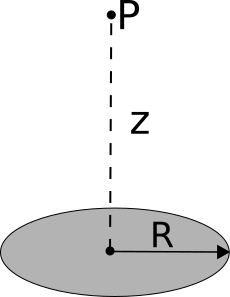
\includegraphics{./images/hw2/disk_of_charge.png}
\caption{Disk of Charge}
\end{figure}

\begin{enumerate}
\def\labelenumi{\arabic{enumi}.}
\tightlist
\item
  Find the electric field at point P, which is a distance \(z\) above
  the center of the disk, by integrating across the surface of the disk.
  \emph{Yes, we know that this field is well-known, but the practice of
  setting up and doing these kinds of integrals is important.} The
  functional form of your solution is a bit complicated and it might be
  tough to see how if its correct - \emph{you can certainly look up the
  answer to check it, but you won't always be able to do that in this
  class (and in life)!}
\item
  If you were very far from this disk, what would you expect the field
  to look like? Use your intuition from PHY 184. Explicitly check the
  limiting form of your solution at very large \(z\) (i.e., when
  \(z >> R\)). \emph{By ``limiting form'', we mean ``how it behaves as a
  function of distance''.} So, don't just say ``it goes to zero'' (if
  that's what you think happens). Tell us how, functionally it vanishes
  (like \(1/z\)? like \(e^{-z}\)? Something else?).
\item
  If you were very close to the disk, what would expect the field too
  look like? Again, use your intuition from PHY 184. Explicitly check
  the limiting form of your solution at very small \(z\) (i.e., when
  \(z << R\)).
\item
  Sketch a qualitatively correct graph of the component of the electric
  field in the \(z\)-direction along the center line. Be sure to include
  both the positive and negative \(z\)-axis in your graph. Your answers
  to parts 2 and 3 might help you here.
\end{enumerate}

\paragraph{5. Ring of charge - Motion of a test
charge}\label{ring-of-charge---motion-of-a-test-charge}

While we spend a large amount of time working with source charges and
the electric fields that they produce, we are ultimately concerned about
their effect on the motion of other charges (so-called ``test
charges''). In this problem, you will work with the electric field due
to a ring of charge to develop an approximate solution for the motion of
a test charge by ``linearizing'' the differential equation that
describes the motion. In working this problem, you will have to dust off
some of your classical mechanics knowledge regarding differential
equations.

Consider a thin ring (positive charge, \(Q\); radius, \(a\)) that has
its central axis directed along the \(x\)-direction as shown.

\begin{figure}[htbp]
\centering
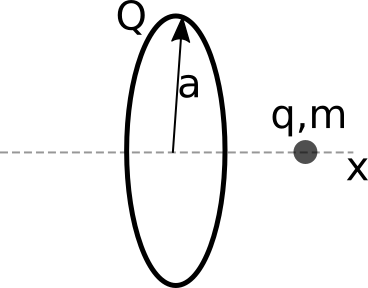
\includegraphics{./images/hw2/ring_w_charge.png}
\caption{Ring of charge}
\end{figure}

A charged ring with these parameters will produce an electric field
along its central axis given by,

\[E_x = \dfrac{1}{4\pi\varepsilon_0}\dfrac{Qx}{\left(x^2+a^2\right)^{3/2}}\]

\begin{enumerate}
\def\labelenumi{\arabic{enumi}.}
\tightlist
\item
  Write down the differential equation that describes the motion of a
  particle with negative charge \(-q\) and mass \(m\) that is carefully
  positioned on the \(x\)-axis. \emph{Note: this particle has a charge
  that is opposite the sign of the ring, so \(q\) is the magnitude of
  the charge of this particle.}
\item
  What kind of motion do you expect to see for this charge? Why? Does
  the differential equation describe that kind of motion? \emph{Hint:
  Consider if this differential equation is analytically tractable
  (i.e., can it be solved in closed form).}
\item
  Consider the situation where the particle is very close to a large
  ring (i.e., where \(x/a\;<<\;1\)). Determine the approximate form of
  the differential equation for this case -- keep only terms that depend
  linearly on \(x\). This is called ``linearizing'' the differential
  equation and makes the solution analytically tractable.
\item
  Solve the differential equation for the case where the particle starts
  from rest at a distance of \(x_0\) from the ring. Sketch the resulting
  motion of the test charge as a function of time. Does your graph agree
  with your intuition about the motion?
\item
  What would happen to the test charge if it was not placed precisely on
  the central axis? Why?
\item
  We have created a Jupyter notebook that models the motion of the test
  charge using both the exact and the approximate differential equation.
  You can \href{../jupyter/HW2-MotionOfTestCharge.ipynb}{download it
  here} (or
  \href{https://github.com/dannycab/phy481msu/blob/gh-pages/jupyter/HW2-MotionOfTestCharge.ipynb}{view
  it here}). By working through this notebook, we expect you to be able
  to explain the output of each model and its assumptions. We also ask
  that you determine under what conditions the approximate model is a
  good one and explain how you know.
\end{enumerate}

\paragraph{6. Finding the electric field of spherical shell using direct
integration}\label{finding-the-electric-field-of-spherical-shell-using-direct-integration}

In this class, you will learn a mathematical technique (Gauss' Law) that
makes solving for the electric field relatively simple in comparison to
direct integration for certain kinds of problems. In this problem, you
will solve for the electric field that can be determined using Gauss'
Law, but you will use direct integration instead. This problem involves
relatively sophisticated integral, which you are free to look up, have
some software solve, or (for the gluttons for pain) solve yourself. The
message here is: when you run across a difficult piece of math, it's ok
to use your resources; just cite your sources!

\begin{enumerate}
\def\labelenumi{\arabic{enumi}.}
\tightlist
\item
  Find the electric field a distance \(z\) above the center of a
  spherical shell of radius \(R\), which carries a uniform surface
  charge density \(\sigma\). Do this by explicit integration (i.e.,
  starting from Griffith's equation 2.7), please. Just treat the case of
  \(z > R\) (\emph{outside} the sphere). Express your answer in terms of
  the total charge \(q\) on the sphere. \emph{Also, be careful, when you
  get a square root, to take the positive root:}
  \(\sqrt{R^2 + z^2 - 2Rz}=(R-z)\) if \(R>z\), but it's \((z-R)\) if
  \(R<z\).
\item
  Check your answer using a units check and your knowledge from PHY 184.
  Briefly discuss what the answer should be outside the sphere. What
  should the answer be inside the sphere and why? \emph{You don't have
  to solve that problem explicitly.}
\end{enumerate}

\emph{Historical note: Newton solved part 1 using geometry (no
calculus!!) This geometric proof is tricky and still excites debate: see
R. Weinstock Am. J. Phys., 52, (1984), p.~883; H. Erlichson, Am. J.
Phys. 58, (1990) p.~882. Newton thought calculus should be kept secret,
and held up publication of Principia until he could work out these
non-calculus proofs. He published calculus much later, about the same
time as Leibniz published his calculus.}
\end{document}
